Wewnątrz tego rodziału znajduje się krótki opis aplikacji służącej do przeprowadzenia badań, oraz implementującej algorytmy zaprezentowane w rozdziale \ref{ssec:algorithms}, specyfikacja zewnętrzna oraz wewnętrzna.
\section{Krótki opis aplikacji}
\label{sec:shortdesc}
Program, który został wykorzystany przy przeprowadzeniu badań został przygotowany jako aplikacja konsolowa. Tego typu aplikacja pozwala na implementację algorytmów, jak również sposobów mierzenia, bez obciążania maszyny o zbędne GUI\footnote{z ang. Graphical User Interface - graficzny interfejs użytkownika}, który może powodować przekłamania względem analizy czasowej i pamięciowej. Aplikacja wykorzystuje celem weryfikacji wpływu czasu połączenia z bazą danych na łączny czas trwania analizy danych wejściowych bazę danych MongoDB, będącej typem bazy NoSQL. W tabeli \ref{tab:nosqlschema} pokazano schemat tabeli z elementami.
\begin{table}[H]
    \centering
    \begin{tabular}{|l|l|}
    \hline
    \textbf{Nazwa} & \textbf{Typ danych} \\ \hline
    \_id           & ObjectId \textit{Unique PK} \\ \hline
    Type           & String              \\ \hline
    CoordX         & Double              \\ \hline
    CoordY         & Double              \\ \hline
    TimeStamp      & String              \\ \hline
    \end{tabular}
    \caption{Schemat tabeli z elementami}
    \label{tab:nosqlschema}
\end{table}
Jak można zaobserwować na schemacie, identyfikator tabeli jest kluczem głównym, unikalnym, generowanym automatycznie przez silnik bazodanowy.\par
Utworzono system działający w następujący sposób:
\begin{itemize}
        \item Podając odpowiednie parametry wejściowe uruchom aplikację.
        \item Skalibruj dane rzeczywiste do formatu układu współrzędnych dwuwymiarowych
        \item Dla każdego punktu oddzielonego punktem posiadającym parametr 'RR' uruchom wybrany algorytm
        \item Zaprezentuj dane wyjściowe na rysunku dla użytkownika
        \item Zapisz dane wyjściowe do pliku
\end{itemize}
Dokładny opis działania każdego z powyższych punktów zaprezentowano w sekcji \ref{sec:internal}.
\section{Wykorzystane narzędzia}
\label{sec:tools}
Projekt został stworzony wykorzystując język programowania \emph{Python} \cite{Python} w wersji 3.7.3. Ten język został wybrany ze względu na jego czytelność oraz modułowość. Kolejnym czynnikiem była prostota w implementacji algorytmów, ze względu na wykorzystanie gotowych funkcjonalności języka Python. Rozważanymi alternatywami był język \emph{F\#} oraz język \emph{R}, Język F\# wykorzystuje platformę .NET, co na pewno ułatwiło by możliwość rozwiązania problemu uczenia maszynowego zaprezentowanego w sekcji \ref{ssec:machinelearningalg}, ze względu na połączenie go z modułem \emph{ML.NET}\footnote{Machine Learning .NET}. Język R w budowie jest bardzo podobny do języka F\#, ale jego kod źródłowy jest otwarty, w przeciwieństwie do F\#\footnote{Należy nadmienić, iż chodzi o standard .NET Framework, a nie .NET Core, dla którego F\# posiada otwarty kod źródłowy} jednak podstawowa znajomość języka Python zadecydowała o wykorzystaniu tej platformy. Wszystkie wymagane moduły oraz sposób użycia opisano w sekcji \ref{ssec:apprequirements}.\par
Praca magisterska została napisana z wykorzystaniem narzędzia \LaTeX\cite{Latex}. Głównym powodem wybrania tego narzędzia jest to, iż prace pisemne tego typu tworzy się łatwo, istnieje dużo rozszerzeń ułatwiających np. wklejanie fragmentów kodu, tworzenie pseudokodu oraz umieszczanie obrazków w dowolnym miejscu oraz formacie. Kolejną zaletą jest darmowość tego pakietu, w przeciwieństwie do pakietu Office firmy Microsoft. Istnieją również rozwiązania darmowe typu OpenOffice, LibreOffice, jednak nie posiadają one takich ułatwień dla prac naukowych. Użyto edytora tekstu Visual Studio Code.\par
Jak wspomniano w sekcji \ref{sec:shortdesc} do stworzenia bazy danych wykorzystano silnik bazodanowy \emph{MongoDB} typu NoSQL. Jest to nierelacyjna baza danych wykorzystująca \textbf{Dokument} jako model danych. Oznacza to, iż dane są zapisywane w formacie BSON\footnote{binary JSON}. Ze względu na wykorzystany typ danych, będący jednym typem, postanowiono użyć tego rozwiązania. Język Python umożliwia w bardzo prosty sposób integrację z bazą danych MongoDB, jak zaprezentowano w sekcji \ref{ssec:connectionDB}.
\section{Specyfikacja zewnętrzna aplikacji}
Celem poniższego podrozdziału jest zaprezentowanie sposobu działania aplikacji, oraz najważniejszych modułów.
\subsection{Parametry wejściowe}
\label{ssec:parameters}
Zadaniem tej sekcji jest przedstawienie dostępnych parametrów wejściowych dla aplikacji.\\
Przez to iż projekt został przygotowany jako program konsolowy, nie posiadający interfejsu użytkownika, konieczne było zaprojektowanie odpowiedniego systemu wprowadzania danych do programu, wraz z wyborem odpowiedniego algorytmu. W tym celu, został przygotowany skrypt uruchomieniowy napisany w języku Powershell. Znajduje się on w głównym katalogu aplikacji. Przykładowa treść została przedstawiona w kodzie \ref{lst:runapp}.\par
\begin{lstlisting}[language=Python, caption=Skrypt uruchomieniowy aplikacji, label={lst:runapp}]
        Set-Location $PSScriptRoot
        python main.py -i '1_01_1311201811.cal' 'ML' -d
        pause
\end{lstlisting}
Jak można zauważyć, druga linia kodu \ref{lst:runapp} odpowiada za uruchomienie aplikacji. Pierwsza linijka ustawia lokalizację środowiska okna w głównym folderze aplikacji, gdyż bez tego domyślną wartością jest wartość \emph{C:/Użytkownicy/nazwaużytkownika}. Ostatnia linia skryptu wymusza na użytkowniku wciśnięcie klawisza żeby zamknąć okno aplikacji.\par
Wszystkie wymagania, żeby uruchomić skrypt zostały podane w sekcji \ref{ssec:apprequirements}.\par
Po nazwie pliku głównego został zaprezentowany przełącznik, który wymaga podania jednej z trzech wartości:
\begin{itemize}
        \item \emph{-i}, odpowiadająca za dalsze działanie aplikacji,
        \item \emph{-h}, wyświetlająca pomoc z aplikacji,
        \item \emph{-a}, pokazującą dostępne algorytmy i wygląd ich parametrów
\end{itemize}
Kolejnym parametrem wejściowym jest nazwa pliku umieszczona w katalogu \emph{/data} w głównym folderze aplikacji. Czwartym parametrem jest algorytm, którym użytkownik chce zbadać wybrany plik wejściowy. Wyróżnia się trzy parametry:
\begin{itemize}
        \item \emph{'ML'}, algorytm wykorzystujący uczenie maszynowe.
        \item \emph{'I-DT'}, algorytm I-DT,
        \item \emph{'I-VT'}, algorytm I-VT
\end{itemize}
Ostatni, \emph{nieobowiązkowy} parametr odpowiada za wybór miejsca, z którego dane mają być wczytywane, \emph{\textbf{-d}} wykonuje połączenie z bazą danych, a \emph{\textbf{-f}} z pliku. W wypadku braku parametru, wykonywana jest ta druga akcja.
\subsection{Format danych wejściowych}
W tej sekcji zaprezentowane zostaną dane wejściowe, otrzymane w wyniku pomiarów z kamery.\par
Wszystkie dane wejściowe zostały umieszczone w folderze \emph{\textbf{/data}} znajdującym się w katalogu głównym aplikacji. Przechowywane one są w formacie \emph{.cal}, który można otworzyć za pomocą dowolnego edytora tekstowego. Zachowaniem przypomina on format \emph{.csv}, z tą różnicą, iż zamiast znaków \emph{;} lub \emph{,} rozdzielających elementy w jednej linii występuje znak specjalny \textbf{/t} odpowiadający jednemu wciśnięciu przycisku TAB na klawiaturze. Przykład pliku wejściowego umieszczono na rysunku \ref{fig:plikwejsciowy}.
\begin{figure}[H]
        \centering
        \captionsetup{justification=centering,margin=2cm}
        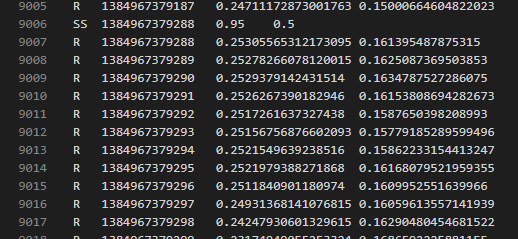
\includegraphics[width=0.8\linewidth]{resources/plikwejsciowy.png}
        \caption{Fragment pliku wejściowego}
        \label{fig:plikwejsciowy}
\end{figure}
Pierwsza kolumna reprezentuje typ danych odczytanych, zawiera ona dwie wartości: \textbf{SS} oraz \textbf{R}. SS oznacza zmianę mierzonego punktu, a wszyskie elementy R oznaczają pomiar. Kolejna kolumna przetrzymuje czas wykonania pomiaru w formacie \emph{UNIX} obliczanym w milisekundach. Jak można zauważyć, pomiar wykonywany jest z częstotliwością 1 ms, przez co odczytane wyniki powinny być dokładne. Trzeci oraz ostatni parametr to nieskalibrowane punkty wejściowe, odpowiednio X i Y. Ich wartości wynoszą od 0 do 1.
\subsection{Format danych wyjściowych}
\blindtext
\subsection{Prezentacja fiksacji}
\blindtext
\section{Specyfikacja wewnętrzna aplikacji}
\label{sec:internal}
W tym podrozdziale przedstawiono informacje dotyczące sposobu implementacji algorytmów przedstawionych w rozdziale \ref{ssec:algorithms}. Przed tymi informacjami przedstawiono moduły języka Python wymagane do uruchomienia aplikacji, oraz sposób ich wykorzystania, jak również opisano metodykę konwersji danych wejściowych na format czytelny dla algorytmów, i sposób połączenia z bazą danych MongoDB.
\subsection{Wymagania aplikacji}
\label{ssec:apprequirements}
Żeby uruchomić skrypt \emph{run.ps1} opisany w sekcji \ref{ssec:parameters} na platformie Windows, należy ustawić parametr \emph{\textbf{ExecutionPolicy}} na wartość \emph{\textbf{Unrestricted}}. Można to wykonać za pomocą polecenia \emph{\textbf{Set-ExecutionPolicy Unrestricted}} w oknie konsoli PowerShell.\par
\subsection{Kalibracja danych wejściowych}
\label{ssec:calibration}
\blindtext
\subsection{Połączenie z bazą danych}
\label{ssec:connectionDB}
\begin{lstlisting}[language=Python, caption=Połączenie z bazą danych, label={lst:connectDB}]
        LOCALHOST = "mongodb://localhost:27017/"
        ...
        myclient = pymongo.MongoClient(LOCALHOST)
        mydb = myclient["mydatabase"]
\end{lstlisting}

\subsubsection{Umieszczenie danych w bazie danych}
Fragment dotyczący umieszczenia danych w bazie danych został zaprezentowany w kodzie \ref{lst:insertDB}. 
\begin{lstlisting}[language=Python, caption=Umieszczenie danych w bazie danych, label={lst:insertDB}]
def initialize_db(pointsList):
    ...
    myclient.drop_database("mydatabase")
    col = mydb["elements"]
    odbcarr = []
    for element in list(pointsList):
            for value in element:
                    doc = collections.OrderedDict()
                    doc['Type'] = value.Type
                    doc['CoordX'] = value.CoordX
                    doc['CoordY'] = value.CoordY
                    doc['TimeStamp'] = value.TimeStamp
                    odbcarr.append(doc)
    col.insert_many(odbcarr)
    ...
\end{lstlisting}
\subsubsection{Wydobycie danych z bazy danych}
\begin{lstlisting}[language=Python, caption=Wydobycie danych z bazy danych, label={lst:getFromDB}]
def getFromDatabase():
    ...
    elements = mydb["elements"].find()
    dataArray = []
    for element in elements:
            item = Data(element['Type'], element['TimeStamp'], element['CoordX'], element['CoordY'])
            dataArray.append(item)
    i = 0
    loopFlag = True
    retList = []
    returnList = []
    while loopFlag:
            for element in dataArray:
                    if i + 1 == len(dataArray):
                            retList.append(dataArray[i])
                            loopFlag = False
                            break
                    if dataArray[i + 1].Type == 'SS':
                            retList.append(dataArray[i])
                            break
                    retList.append(dataArray[i])
                    i += 1
            i += 1
            returnList.append(retList)
            retList = []
    ...
    \end{lstlisting}
\subsection{Algorytm I-VT}
\blindtext
\subsection{Algorytm I-DT}
\begin{lstlisting}[language=Python, caption=Kod algorytmu I-DT, label={lst:idt}]
def calculateIdtAlgorithm(pointsList):
        start = time.process_time()
        i = 0
        timeStart = int(pointsList[0].TimeStamp)
        windowList = []
        coordXList = []
        coordYList = []
        countPoints = len(pointsList)
        while i < countPoints - 1:
        if pointsList[i].Type == 'SS':
                i += 1
                continue
        currTime = int(pointsList[i].TimeStamp)
        while currTime - timeStart <= constants.WINDOW_TIME_THRESHOLD:
                windowList.append(pointsList[i])
                i += 1
                if i >= countPoints:
                break
                currTime = int(pointsList[i].TimeStamp)
        if i >= countPoints:
                break
        if len(windowList) > 1:
                Dispersion = (max(maxX.CoordX for maxX in windowList) - min(minX.CoordX for minX in windowList)) + (max(maxY.CoordY for maxY in windowList) - min(minY.CoordY for minY in windowList))
        while len(windowList) > 1:
                if Dispersion <= constants.DISPERSION_THRESHOLD and len(windowList) > 1:
                while (Dispersion < constants.DISPERSION_THRESHOLD):
                        windowList.append(pointsList[i])
                        i += 1
                        if i >= countPoints:
                        break
                        Dispersion = (max(maxX.CoordX for maxX in windowList) - min(minX.CoordX for minX in windowList)) + (max(maxY.CoordY for maxY in windowList) - min(minY.CoordY for minY in windowList))
                if i >= countPoints:
                        break
                coordXList.append(sum(sumX.CoordX for sumX in windowList) / len(windowList))
                coordYList.append(sum(sumY.CoordY for sumY in windowList) / len(windowList))
                else:
                windowList.pop(0)
        if i <= countPoints - 1:
                timeStart = int(pointsList[i].TimeStamp)
        end = time.process_time()
        return coordXList, coordYList, end - start, len(coordXList)
\end{lstlisting}
\subsection{Algorytm wykorzystujący uczenie maszynowe}
\label{ssec:machinelearningalg}
\blindtext
